% Copyright (C) 2021  Agenium Scale
% 
% This program is free software: you can redistribute it and/or modify
% it under the terms of the GNU General Public License as published by
% the Free Software Foundation, either version 3 of the License, or
% (at your option) any later version.
% 
% This program is distributed in the hope that it will be useful,
% but WITHOUT ANY WARRANTY; without even the implied warranty of
% MERCHANTABILITY or FITNESS FOR A PARTICULAR PURPOSE.  See the
% GNU General Public License for more details.
% 
% You should have received a copy of the GNU General Public License
% along with this program.  If not, see <https://www.gnu.org/licenses/>.

\documentclass[a4paper,11pt]{article}
\usepackage[utf8]{inputenc}
\usepackage[T1]{fontenc}
\usepackage[right=2cm,left=2cm,bottom=2cm,top=2.5cm,headheight=2em]{geometry}
\usepackage[ddmmyyyy]{datetime}
\usepackage{xcolor}
\usepackage[colorlinks,linkcolor=black,urlcolor=blue]{hyperref}
\usepackage{listings}
\usepackage{lstautogobble}
\usepackage{tabularx}
\usepackage{csvsimple}
\usepackage{graphicx}
\usepackage{fancyhdr}
\usepackage{pgf}
\usepackage{pgffor}
\usepackage{mdframed}
\usepackage{amsmath}

% sans-serif font ("Computer Modern Sans") instead of roman font
\renewcommand{\rmdefault}{\sfdefault}
% "CourrierNew" font (for code listing)
\renewcommand{\ttdefault}{pcr}

\lstset{
	basicstyle=\small\ttfamily,
	backgroundcolor=\color{white},
	breaklines=true,
	breakatwhitespace=true,
	tabsize=2,
	frame=single,
	rulecolor=\color{black},
	keywordstyle=\color{blue}\bfseries,
	stringstyle=\color{orange},
	showstringspaces=false,
	commentstyle=\footnotesize\color{darkgreen},
	keepspaces=true,
	extendedchars=true,
	numbers=none,
	numberstyle=\tiny\color{lightgray},
	stepnumber=1,
	escapeinside={(@}{@)},
	autogobble=true,
	literate=
		{á}{{\'a}}1 {é}{{\'e}}1 {í}{{}}1 {ó}{{\'o}}1 {ú}{{\'u}}1
		{Á}{{\'A}}1 {É}{{\'E}}1 {Í}{{\'I}}1 {Ó}{{\'O}}1 {Ú}{{\'U}}1
		{à}{{\`a}}1 {è}{{\`e}}1 {ì}{{\`i}}1 {ò}{{\`o}}1 {ù}{{\`u}}1
		{À}{{\`A}}1 {È}{{\'E}}1 {Ì}{{\`I}}1 {Ò}{{\`O}}1 {Ù}{{\`U}}1
		{ä}{{\"a}}1 {ë}{{\"e}}1 {ï}{{\"i}}1 {ö}{{\"o}}1 {ü}{{\"u}}1
		{Ä}{{\"A}}1 {Ë}{{\"E}}1 {Ï}{{\"I}}1 {Ö}{{\"O}}1 {Ü}{{\"U}}1
		{â}{{\^a}}1 {ê}{{\^e}}1 {î}{{\^i}}1 {ô}{{\^o}}1 {û}{{\^u}}1
		{Â}{{\^A}}1 {Ê}{{\^E}}1 {Î}{{\^I}}1 {Ô}{{\^O}}1 {Û}{{\^U}}1
		{œ}{{\oe}}1 {Œ}{{\OE}}1 {æ}{{\ae}}1 {Æ}{{\AE}}1 {ß}{{\ss}}1
		{ç}{{\c c}}1 {Ç}{{\c C}}1 {ø}{{\o}}1 {å}{{\r a}}1 {Å}{{\r A}}1
		{€}{{e}}1 {£}{{\pounds}}1 {«}{{\guillemotleft}}1
		{»}{{\guillemotright}}1 {ñ}{{\~n}}1 {Ñ}{{\~N}}1 {¿}{{?`}}1
}


\pagestyle{fancy}
\renewcommand{\headrulewidth}{0pt}
\renewcommand{\footrulewidth}{0pt}
\fancyhf[CLRHF]{}
\fancyhf[LH]{\includegraphics[height=\dimexpr(\headheight-.5em)\relax]
                             {logo_agenium_scale}}
\fancyhf[CF]{\thepage}

\date{\today}
\author{\includegraphics[width=20em]{logo_agenium_scale}}
\title{EFISPEC3D/NSIMD Benchmarks __ENV_TITLE__}

\newcommand{\efispec}{EFISPEC3D}
\newcommand{\nsimd}{NSIMD}
\newcommand{\cpu}{CPU}
\newcommand{\ageniumscale}{AGENIUM SCALE}

\begin{document}
\maketitle%
\vspace*{\fill}%
\noindent%
\textbf{\ageniumscale{}}\\
Rue Noetzlin\\
Batiment 660, Digiteo Labs\\
91 190 Gif-sur-Yvette\\
01 69 15 32 32\\
\href{mailto://contact@numscale.com}{contact@numscale.com}\\
\href{https://agenium-scale.com}{https://agenium-scale.com}\\
\thispagestyle{empty}
\clearpage
%
\thispagestyle{empty}
\tableofcontents
\newpage

\subsection*{About}%
\label{sec:about}

This document is a \textbf{technical} report of the \efispec{} benchmarks
performed by \ageniumscale{} on __COMPUTER__. The aim
is to give a quick idea of how vector code using \nsimd{} performs against
other versions.

The document was automatically generated on \today. No human was involved in
running the benchmarks. There are many benchmarks and not all of them can be
checked by a human. Therefore if you find weird results, fell free to contact
\ageniumscale{} at \href{mailto://contact@numscale.com}{contact@numscale.com}.
If you want us to run benchmarks on a machine you own, feel free to contact us
at \href{mailto://contact@numscale.com}{contact@numscale.com} to see whether
and how we can help you.

This document is meant to be read by software developers. The explanations
provided in the following sections are not intended to be detailed. We assume
that the reader has the knowledge required to understand the present document.
If you have any relevant question feel free to contact us at
\href{mailto://contact@numscale.com}{contact@numscale.com}.

\begin{mdframed}{
  \textbf{Disclaimer}

  All the information, including technical and engineering data, processes,
  and results, presented in this document has been prepared carefully in
  order to present an accurate vision of NSIMD's performance. However, the
  reader is informed that the hardware and software environment may affect
  NSIMD's performance and present results that are distinct from those
  presented herein.

  Thus, \ageniumscale{} does not guarantee in any way the accuracy or
  completeness of the results presented, which are provided for illustrative
  purposes only. The terms used in this document shall not be construed as
  offering any guarantee of result, purpose, and more generally no warranty of
  any kind.

  For more details on our commitments, we refer you to the NSIMD license
  agreement which sets out the scope of our commitments.
}\end{mdframed}

\section{Setup}%
\label{sec:setup}

\subsection{Details on \efispec{}}

\subsubsection{Introduction to \efispec{}}

Physics-based three-dimensional numerical simulations are becoming more
predictive and have already become essential in geosciences. In geophysics,
simulations at scale with a very fine resolution, including uncertainty
quantification procedures are crucial to provide the relevant physical
parameters for forward modeling of seismic wave propagation. The forward wave
propagation problem is governed by the elastodynamic equations of motion:

\begin{equation}
\label{equ:eom}
  \rho \ddot{u_{i}} = f_{i} + \tau_{ij,j},
\end{equation}

\noindent where $\rho$ is the material density; $\ddot{u_{i}}$ is the $i$-th
component of the second time-derivative of the displacement $u_{i}$;
$\tau_{ij,j}$ is the spatial derivative of the stress tensor component
$\tau_{ij}$ with respect to $x_j$; $ f_{i}$ is the $i$-th component of the body
force.

From the numerical point of view, several methods have been successfully used
for the simulation of elastic wave propagation in three-dimensional domains.
Finite-difference methods (FDM), classical or spectral finite-element methods
(FEM and SEM) have been introduced last few years for this class of problems.
Interested readers could refer to~\cite{Moczo} for further details on these
approaches.  Due to its numerical efficiency, the spectral finite-element
method~(SEM) is routinely used for seismic simulations~(\cite{Kom97}). As an
example, SPECFEM3D is a major software package dedicated to seismic wave
modeling. The code implements the SEM  leading to breakthroughs in
computational geophysics on multi-petascale systems~(\cite{TsuboiAMPKT16}). The
weak form of eq. \ref{equ:eom}  is expressed in eq. \ref{equ:weak-formulation},
is solved in its discretized form by using this method.

\begin{equation}
\label{equ:weak-formulation}
\int _{\Omega} \rho \mathbf{v}^{_T} \cdot \mathbf{\ddot{u}} \, d\Omega =
  \int _{\Omega}  \boldsymbol{\epsilon}(\mathbf{v})^{_T} \colon
    \boldsymbol{\tau} \, d\Omega 
- \int _{\Omega}  \mathbf{v}^{_T} \cdot \mathbf{f} \, d\Omega
- \int _{\Gamma}  \mathbf{v}^{_T} \cdot \mathbf{T} \, d\Gamma
\end{equation}

where $\Omega$ and $\Gamma$ are the volume and the surface area of the domain
under study, respectively; $\boldsymbol{\epsilon}$ is the virtual strain tensor
related to the virtual displacement vector $\mathbf{v}$; $\mathbf{f}$ is the
body force vector and $\mathbf{T}$ is the traction vector acting on $\Gamma$.
Superscript $T$ denotes the transpose, and a colon denotes the contracted
tensor product.

As reported in ~(\cite{RotenCODWSWM16,TsuboiAMPKT16,BreuerHB16}), explicit
parallel elastodynamics application usually exhibits very good weak and strong
scaling up to several tens of thousands of cores. But if we focus on SIMD-level
optimizations, the compiler performance plays a major role and recent studies
have underlined the limited impact of automatic vectorization
~\cite{Sornet20171083,Kruzel20132030}.  Most of the time, the complexity of the
computational workflows limit the efficacy of automatic optimization
mechanisms. 

For the Spectral-element method, it is admitted that the summation of the
element contributions~(assembly phase) represents a major bottleneck. This is
coming both from the shared values between neighboring elements and the
inherent indirection for data accesses induced by this approach.

The complexity of the internal loop might also be a blocker for the compiler.
Despite representing as much as 80\% of the total elapsed time, only hand-tuned
implementations have been able to fully vectorize the computation of internal
forces.

\subsubsection{Scalar version}

The kernel is composed of four loop levels. The outermost one iterates over
elements.  For each element, we perform the three following steps: 1) gathering
points of the element, 2) computing internal forces, 3) assembly step: element
contribution is updated. Each of these steps consists of three nested loops to
iterate along the three directions of each element.

Gathering points for each element consists in copying values from a global
array to a local array following an indirection array.  These indirections are
required since element borders overlap: one point may be shared by up to eight
elements (corners).  Points are not replicated in order to reduce memory
footprint and avoid multiple updates at step 3.  The local array is relatively
small and is likely to fit and stay into the L1 cache along the two other
steps.  For example, at order 4, the element consists of a block of 5x5x5
points, each point containing three floating point values, thus a total of
1.5kB per element.

Internal forces are computed by traversing the element along the three
directions, multiplying point values by Lagrangian coefficients and
accumulating the results.  Thus, it essentially consists of additions and
multiplications which are likely to be merged into FMA (Fused Multiply Add)
instructions.

Finally, results are to be stored back to the global array with the same
indirection pattern as for the gathering step.

\subsubsection{Vectorization approach}

A common approach suited for vectorizing most algorithms is to vectorize the
innermost loop.  For our kernel, the number of iterations for the three inner
loops depends on the considered order.  At order 4, the innermost loop only
performs five iterations, which is enough to feed 128-bit SIMD units, but not
enough to feed larger 512-bit SIMD units.  It is possible to fuse the inner
loops to bring more vectorization opportunities.  However, this approach has
several drawbacks:
\begin{enumerate}
  \item It does not exactly match the register length in the general case and
        thus still requires some scalar or masked instructions.
  \item It requires irregular accesses to data since data in the same register
        may not be contiguous following the element structure.
  \item It breaks the code organization making it harder for the developer to
        read/modify/maintain.
  \item It is not possible to write a single generic code independent from the
        considered order and from the SIMD unit width.
\end{enumerate}

A much simpler approach consists of vectorizing the outermost loop, thus
applying the same computation over several elements at the same time.  It
allows us to solve the above problems.  The SIMD unit width determines the
number of elements considered at the same time.  With a 128-bit SIMD
instruction set, we can store four single precision floating point values into
a single register, thus we can process four elements at the same time. Only a
few remaining elements may be computed the scalar way with, thus requiring to
keep a scalar version of the code after the vectorized one.  With masked
instructions provided by some SIMD extensions, the remaining elements are
processed with the same code.  Another advantage of this approach is that the
code organization stays the same.  Instead of considering scalar floating point
values, we consider vectors of floating point values, and arithmetic
instructions are exactly the same but are applied on these vectors.

\subsection{Benchmark Organisation}

Each comparison requires specific \efispec{} binaries that have been tailored
for the vector instruction set chosen. We compiled a set of binaries using the
hand-written intrinsics versions of the code and a set using \nsimd{}.

The next chapter present the graph comparing the running times coming from
the different runs of the \efispec{} binaries each of which compiled with its
own set of SIMD instructions.

\subsection{Protocol}

For each SIMD extension, \efispec{} is run. Note that the goal of this document
is \emph{not} to measures the performances of a particular compiler or CPU. The
\emph{only} goal is to measure NSIMD performances against \efispec{}'s versions
of hand-written intrinsics. Note that the code is not multi-threaded as our
goal is to run single-core benchmark to measure the impact of the use of SIMD
extensions.

\subsubsection{CPU}
\lstinputlisting{cpu.info}

\subsubsection{RAM}
\lstinputlisting{memory.info}

\subsubsection{System}
\lstinputlisting{uname.info}

\subsubsection{Compiler}
\lstinputlisting{compiler.info}

\subsubsection{C standard library}
\lstinputlisting{libc.info}
 
\newpage
\section{Comparison graph}

The following graph represent to running time of all \efispec{} binaries that
have been run in this benchmark. Timings are in milliseconds.

\begin{center}
  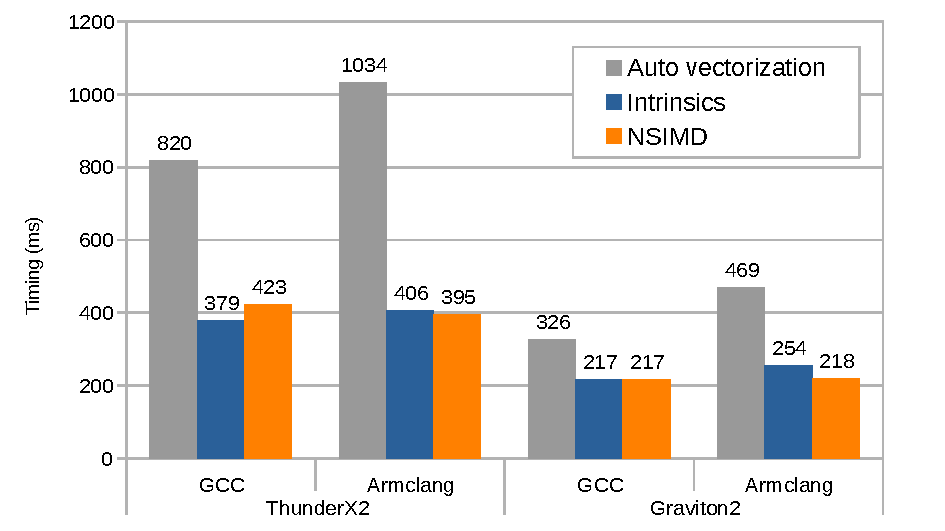
\includegraphics[width=\textwidth]{timings.pdf}
\end{center}

\newpage
\bibliography{biblio}
\addcontentsline{toc}{section}{References}
\bibliographystyle{alpha}

\end{document}
